%----------------------------------------------------------------------------------------
\begin{frame}
  \frametitle{2D Laminar flow around a cylinder}
  \textbf{Problem setting:}
  \begin{itemize}
 	\item Widely used benchmark.
  	\item $Re=100$. 
  	\item Time convergence.
  	\item Drag and Lift coefficients.
  \end{itemize}
  \begin{figure}
   \centering	  
   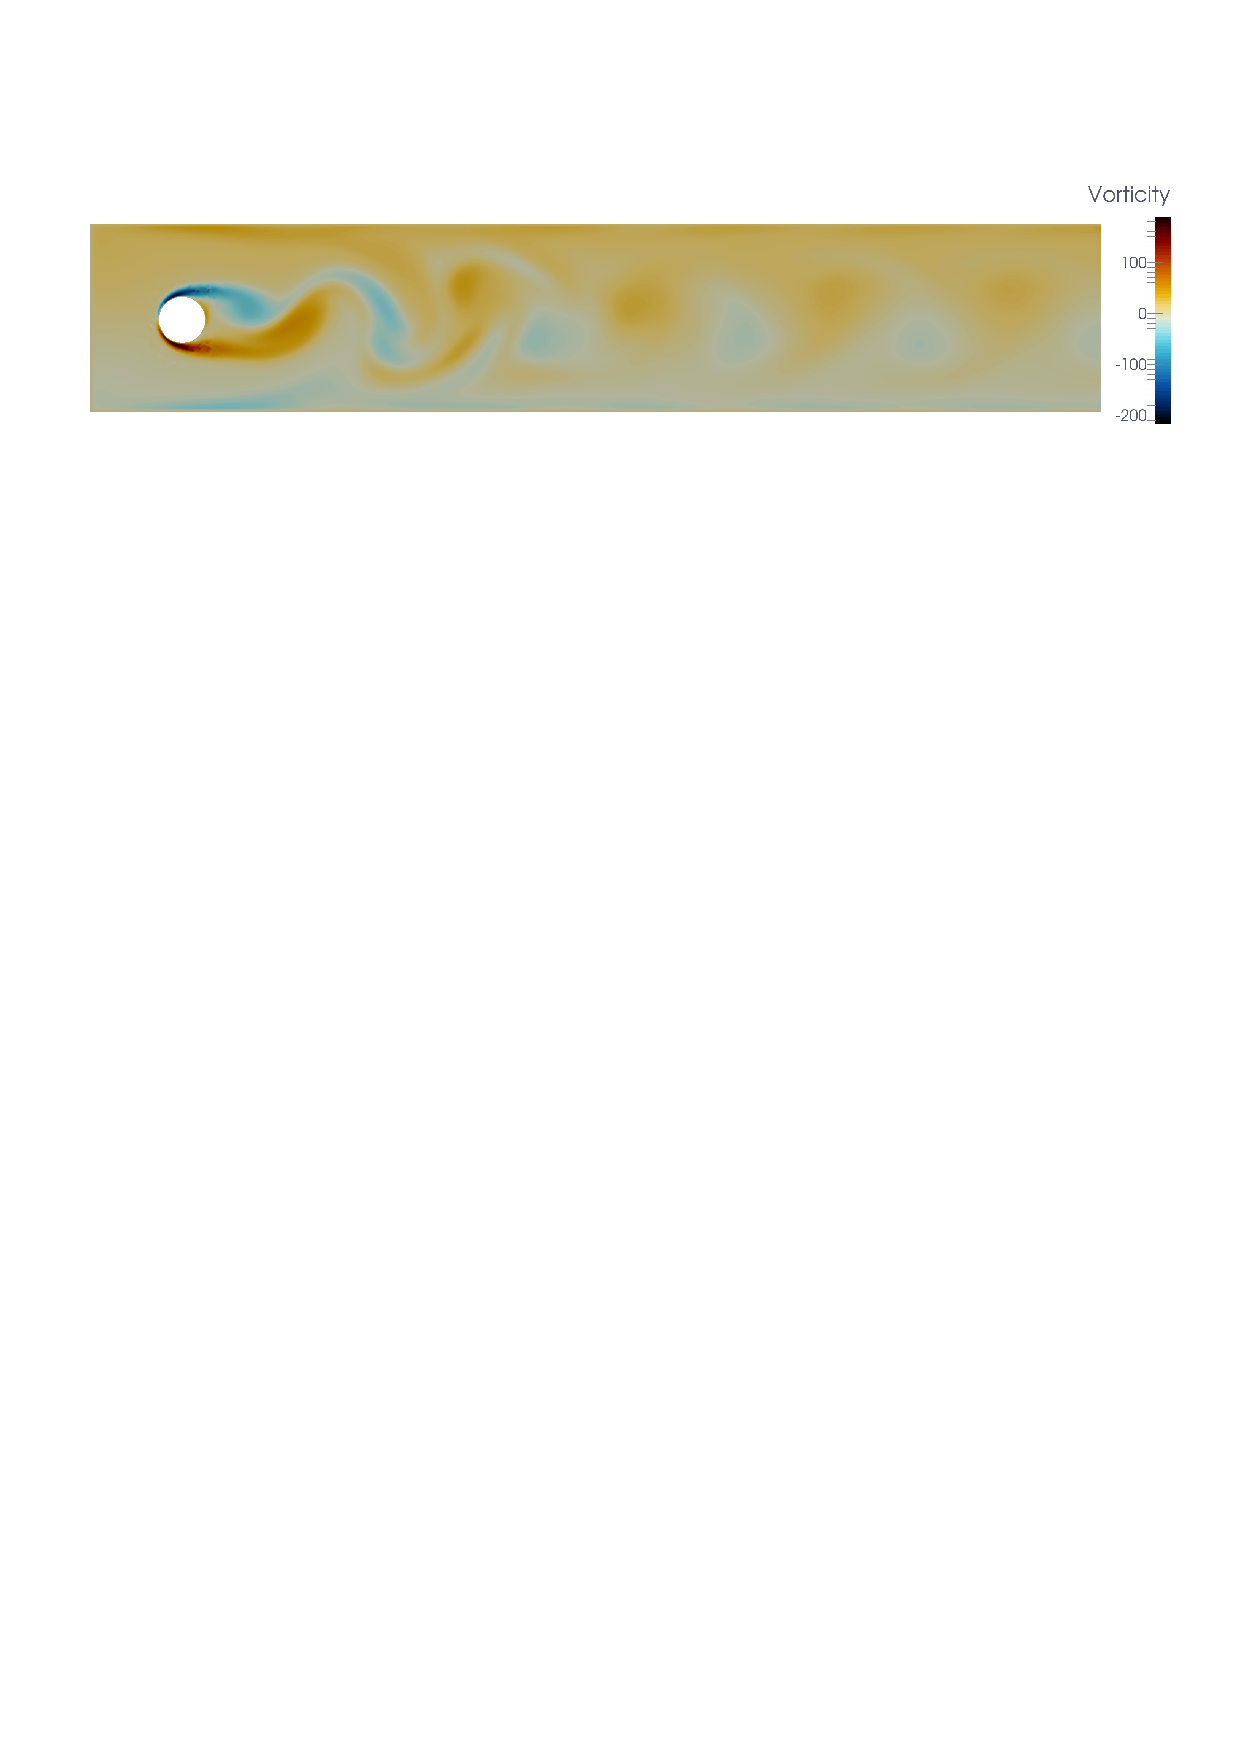
\includegraphics[clip=true,trim=1.5cm 22.5cm 1cm 3cm,width=1.0\textwidth]{Figures/vorticity}
     \caption{Vorticity field at $t=8.0$.}
     \label{fig:Cyl_vorti}
  \end{figure}
\end{frame}
%----------------------------------------------------------------------------------------
\begin{frame}
\frametitle{2D Laminar flow around a cylinder}
\only<1>{
\textbf{Implicit convection:}
\begin{figure}[h!]
  \centering
  \subfigure[Velocity convergence]{\label{fig:IMEX_RK_vel_cyl_impl_expl}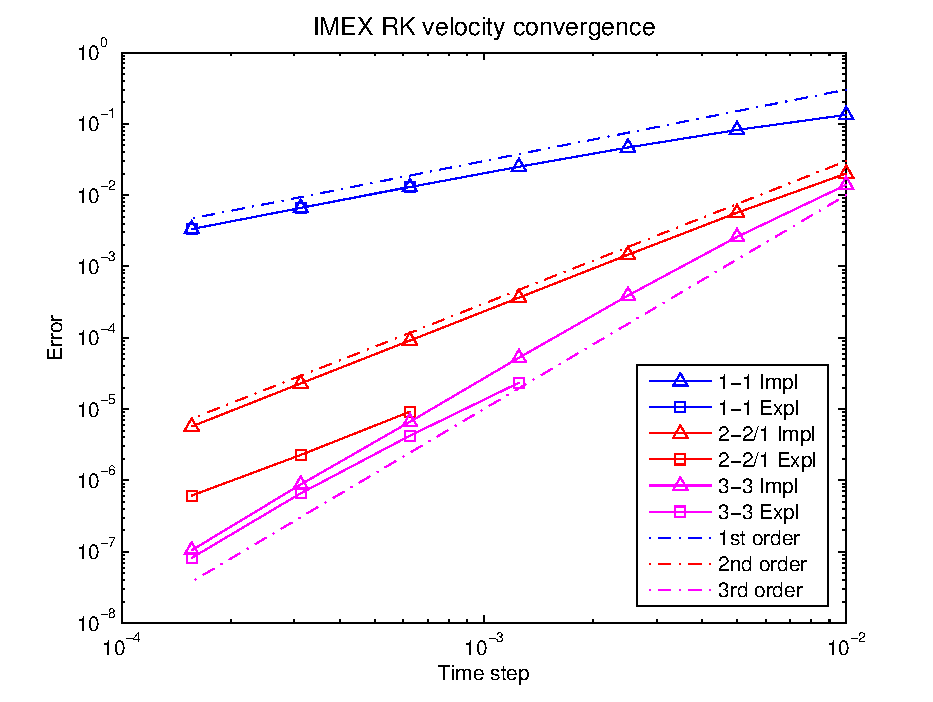
\includegraphics[width=0.49\textwidth]{Figures/vel_impl_expl}}    
  \subfigure[Pressure convergence]{\label{fig:IMEX_RK_pre_cyl_impl_expl}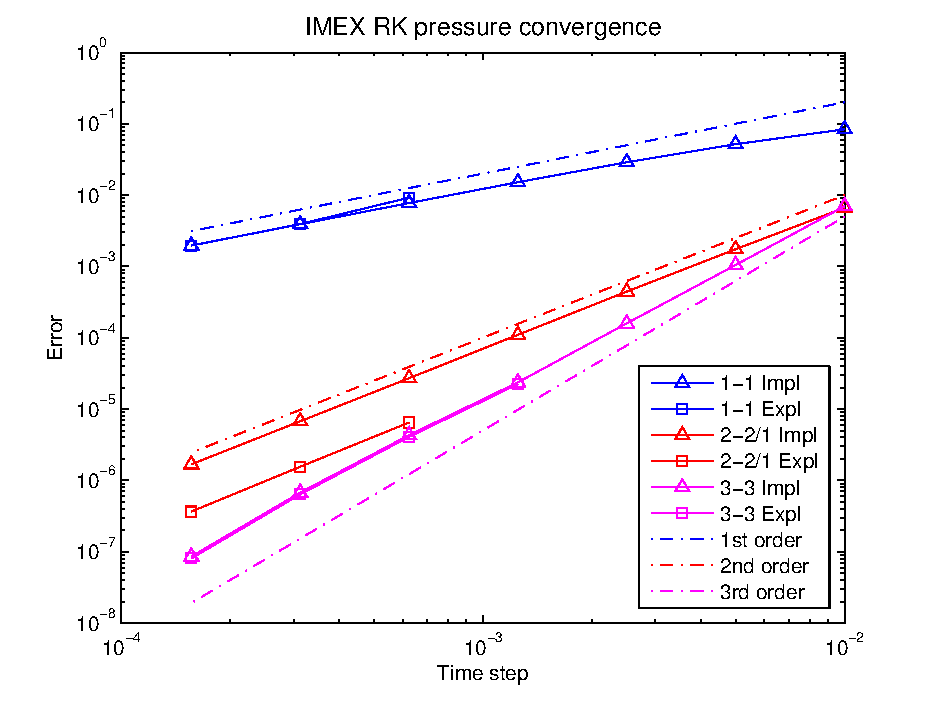
\includegraphics[width=0.49\textwidth]{Figures/pre_impl_expl}}
  \caption{Fully implicit and IMEX-SRK convergence rate comparison.}
  \label{fig:IMEX_RK_cyl_conv_impl_expl}
\end{figure}}
\only<2>{
\textbf{Adaptive time stepping:}
\begin{figure}[h!]
  \centering
  \subfigure[Time step evolution]{\label{fig:IMEX_RK_cyl_adp_dt}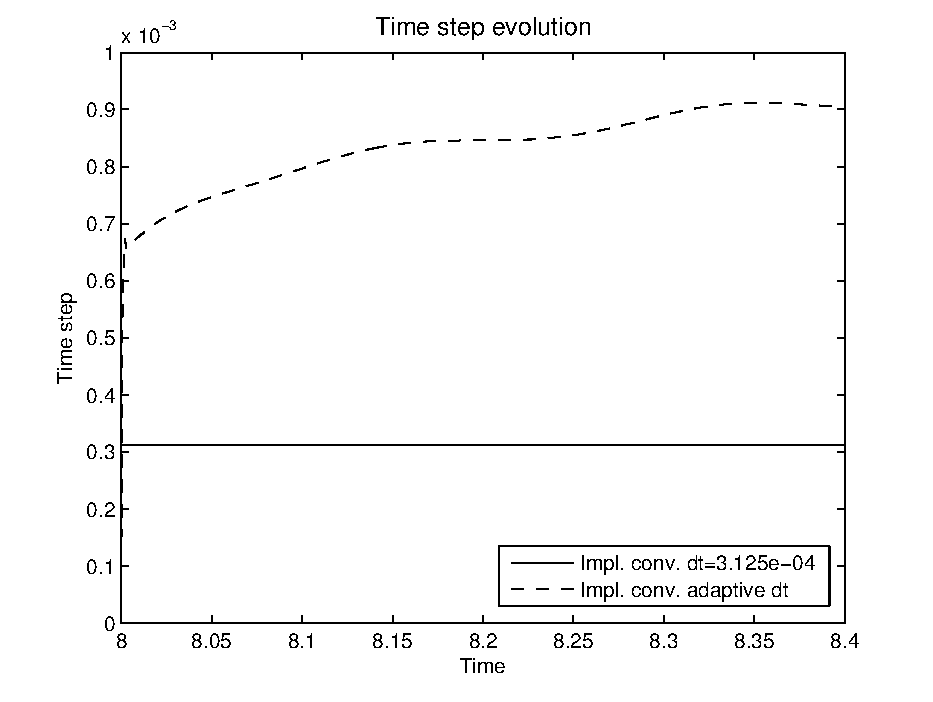
\includegraphics[width=0.49\textwidth]{Figures/time_step}}    
  \subfigure[Lift coefficient (zoom)]{\label{fig:IMEX_RK_cyl_adp_lift}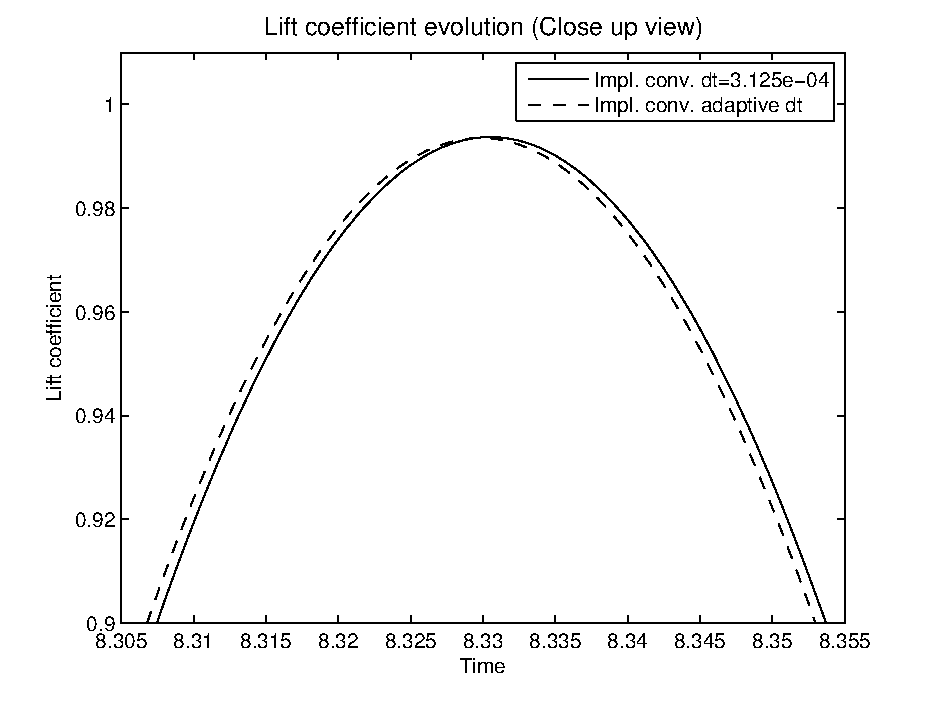
\includegraphics[width=0.49\textwidth]{Figures/lift_close}}
  \caption{Adaptive time stepping.}
  \label{fig:IMEX_RK_cyl_adp}
\end{figure}}
\end{frame}


